% \LaTeX-Main\
%% The LaTeX package tcolorbox - version 4.22 (2019/11/15)
%% tcolorbox-tutorial-poster.tex: a tutorial for poster creation with tcolorbox
%%
%% -------------------------------------------------------------------------------------------
%% Copyright (c) 2006-2019 by Prof. Dr. Dr. Thomas F. Sturm <thomas dot sturm at unibw dot de>
%% -------------------------------------------------------------------------------------------
%%
%% This work may be distributed and/or modified under the
%% conditions of the LaTeX Project Public License, either version 1.3
%% of this license or (at your option) any later version.
%% The latest version of this license is in
%%   http://www.latex-project.org/lppl.txt
%% and version 1.3 or later is part of all distributions of LaTeX
%% version 2005/12/01 or later.
%%
%% This work has the LPPL maintenance status `author-maintained'.
%%
%% This work consists of all files listed in README
%%
% arara: pdflatex: { shell: yes }
% arara: pdflatex: { shell: yes }
\documentclass[12pt]{article}

\usepackage[a3paper,landscape]{geometry}
\usepackage{lipsum}
\usepackage{lmodern}
\usepackage{enumerate}

\usepackage[poster]{tcolorbox}
\tcbuselibrary{minted} % <- replace by \tcbuselibrary{listings}, if minted does not work for you

\pagestyle{empty}


\newtcolorbox[auto counter]{guide}[1][]{enhanced jigsaw,inherit height,
  colback=red!5,opacityback=0.9,colframe=red,title=Poster Tutorial \#\thetcbcounter,
  grow to left by=8mm,grow to right by=8mm,
  arc is angular,arc=3mm,
  fonttitle=\bfseries\large,
  fuzzy halo=4mm with blue!50!red,#1
}

\tcbset{
  mylisting/.style={enhanced jigsaw,size=minimal,toprule=0.5mm,bottomrule=0.5mm,boxsep=2mm,oversize,
  colback=white,opacityback=0.75,listing only}
}

\newtcblisting{guidelisting}[1]{mylisting,#1}


\begin{document}

%%%%%%%%%%%%%%%%%%%%%%%%%%%%%%%%%%%%%%%%%%%%%%%%%%%%%%%%%%%%%%%%%%%%%%%%%%%%%%%


\begin{tcbposter}[
  coverage = {spread},
  poster   = {showframe,columns=4,rows=5},
]


\begin{posterboxenv}[blankest]{column=2,span=2,at=middle}
\begin{guide}[toptitle=3mm,before title={\begin{center}
Thomas F.~Sturm\\
\Large A Tutorial for Poster Creation with Tcolorbox
\end{center}}]
Welcome to the poster tutorial!
\tcbline
We start at the very begin with an empty poster.\par\medskip
In this tutorial, we use A3 sized paper in landscape format which can
be set up with the \texttt{geometry} package.
Naturally, we need the \texttt{tcolorbox} package with at least the
\texttt{poster} library loaded.\par
At begin, we only choose the number of columns (4) and rows (5) and
we display a help grid.\par\medskip

\begin{guidelisting}{}
\documentclass[12pt]{article}
\usepackage[a3paper,landscape]{geometry}
\usepackage[poster]{tcolorbox}
\pagestyle{empty}

\begin{document}
\begin{tcbposter}[
  coverage = {spread},
  poster   = {showframe,columns=4,rows=5},
]
% Here, we insert the poster content later
\end{tcbposter}
\end{document}
\end{guidelisting}
\end{guide}
\end{posterboxenv}

\end{tcbposter}



%%%%%%%%%%%%%%%%%%%%%%%%%%%%%%%%%%%%%%%%%%%%%%%%%%%%%%%%%%%%%%%%%%%%%%%%%%%%%%%

\begin{tcbposter}[
  coverage = {
      spread,
      interior style={top color=yellow,bottom color=yellow!50!red},
      watermark text={\LaTeX\ Poster},
      watermark color=yellow,
  },
  poster   = {showframe,columns=4,rows=5},
]

\begin{posterboxenv}[blankest]{column=2,span=2,above=bottom}
\begin{guide}
Now, we put in some fancy settings to the poster \texttt{coverage}.\par
Also, some more packages are loaded for the future poster content.
\par\medskip

\begin{guidelisting}{}
\documentclass[12pt]{article}
\usepackage[a3paper,landscape]{geometry}
\usepackage{lipsum}
\usepackage{lmodern}
\usepackage{enumerate}
\usepackage[poster]{tcolorbox}
\tcbuselibrary{minted} % <- replace by \tcbuselibrary{listings}, if minted does not work for you
\pagestyle{empty}

\begin{document}
\begin{tcbposter}[
  coverage = {
      spread,
      interior style={top color=yellow,bottom color=yellow!50!red},
      watermark text={\LaTeX\ Poster},
      watermark color=yellow,
  },
  poster   = {showframe,columns=4,rows=5},
]
% Here, we insert the poster content later
\end{tcbposter}
\end{document}
\end{guidelisting}
\end{guide}
\end{posterboxenv}

\end{tcbposter}



%%%%%%%%%%%%%%%%%%%%%%%%%%%%%%%%%%%%%%%%%%%%%%%%%%%%%%%%%%%%%%%%%%%%%%%%%%%%%%%

\begin{tcbposter}[
  coverage = {
      spread,
      interior style={top color=yellow,bottom color=yellow!50!red},
      watermark text={\LaTeX\ Poster},
      watermark color=yellow,
  },
  poster   = {showframe,columns=4,rows=5},
]

%----
\posterbox{name=title,column=1,span=3,below=top}{
  \resizebox{18cm}{!}{\bfseries\Huge My Important Project}\\[3mm]
  Hans.Mustermann@deepthought.university
}

%----
\posterbox[adjusted title=References]{name=references,column=2,span=1.5,above=bottom}{
}

%----
\posterbox[adjusted title=Process]{name=process,column=2,span=2,above=references}{
}

%----
\posterbox[adjusted title=Project Description]{name=project,
    sequence=1 between title and bottom then 2 between title and process}{
}

%----
\posterbox[adjusted title=Central Picture]
  {name=picture,column=3,between=title and process}{}

%----
\begin{posterboxenv}[adjusted title=Core Algorithm]
  {name=algorithm,column=4,between=top and references}
\end{posterboxenv}

%----
\posterbox[adjusted title=Contact]
    {name=contact,column*=4,span=1.5,between=process and bottom}{
}

\begin{posterboxenv}[blankest]{column=3,span=2,at=middle}
\begin{guide}
It is time to fill boxes into the \texttt{poster} environment.
This is the most crucial part of your poster creation, because you have
to decide about the general contents and the base design.\par
But, as you can see in the listing below, the boxes are placed with
relative positions to each other and the sizes are able to change
automatically.
\par\medskip

\begin{guidelisting}{}
%...
\posterbox{name=title,column=1,span=3,below=top}{
  \resizebox{18cm}{!}{\bfseries\Huge My Important Project}\\[3mm]
  Hans.Mustermann@deepthought.university
}

\posterbox[adjusted title=References]{name=references,column=2,span=1.5,above=bottom}{}

\posterbox[adjusted title=Process]{name=process,column=2,span=2,above=references}{}

\posterbox[adjusted title=Project Description]{name=project,
    sequence=1 between title and bottom then 2 between title and process}{}

\posterbox[adjusted title=Central Picture]
  {name=picture,column=3,between=title and process}{}

\posterbox[adjusted title=Core Algorithm]
  {name=algorithm,column=4,between=top and references}{}

\posterbox[adjusted title=Contact]
    {name=contact,column*=4,span=1.5,between=process and bottom}{}
%...
\end{guidelisting}
\medskip
The \texttt{project} box is made breakable. Note the two parts
\texttt{project1} and \texttt{project2} where the second part is
denoted by a placeholder.
\end{guide}
\end{posterboxenv}
\end{tcbposter}



%%%%%%%%%%%%%%%%%%%%%%%%%%%%%%%%%%%%%%%%%%%%%%%%%%%%%%%%%%%%%%%%%%%%%%%%%%%%%%%
\begin{tcbposter}[
  coverage = {
      spread,
      interior style={top color=yellow,bottom color=yellow!50!red},
      watermark text={\LaTeX\ Poster},
      watermark color=yellow,
  },
  poster   = {showframe=false,columns=4,rows=5},
  boxes    = {
      enhanced standard jigsaw,sharp corners=downhill,arc=3mm,boxrule=1mm,
      colback=white,opacityback=0.75,colframe=blue,
      title style={left color=black,right color=cyan},
      fonttitle=\bfseries\Large\scshape
   }
]

%----
\posterbox{name=title,column=1,span=3,below=top}{
  \resizebox{18cm}{!}{\bfseries\Huge My Important Project}\\[3mm]
  Hans.Mustermann@deepthought.university
}

%----
\posterbox[adjusted title=References]{name=references,column=2,span=1.5,above=bottom}{
}

%----
\posterbox[adjusted title=Process]{name=process,column=2,span=2,above=references}{
}

%----
\posterbox[adjusted title=Project Description]{name=project,
    sequence=1 between title and bottom then 2 between title and process}{
}

%----
\posterbox[adjusted title=Central Picture]
  {name=picture,column=3,between=title and process}{}

%----
\begin{posterboxenv}[adjusted title=Core Algorithm]
  {name=algorithm,column=4,between=top and references}
\end{posterboxenv}

%----
\posterbox[adjusted title=Contact]
    {name=contact,column*=4,span=1.5,between=process and bottom}{
}

\begin{posterboxenv}[blankest]{column=3,span=2,at=middle}
\begin{guide}
As next step, we choose some nice settings for all the boxes. These
global settings are applied using the \texttt{boxes} option of
the poster.\par
Also, we do not need the auxiliary frame lines anymore and we set
\texttt{showframe=false}.
\par\medskip

\begin{guidelisting}{}
%...
\begin{tcbposter}[
  coverage = {
      spread,
      interior style={top color=yellow,bottom color=yellow!50!red},
      watermark text={\LaTeX\ Poster},
      watermark color=yellow,
  },
  poster   = {showframe=false,columns=4,rows=5},
  boxes    = {
      enhanced standard jigsaw,sharp corners=downhill,arc=3mm,boxrule=1mm,
      colback=white,opacityback=0.75,colframe=blue,
      title style={left color=black,right color=cyan},
      fonttitle=\bfseries\Large\scshape
   }
]
%...
\end{guidelisting}
\end{guide}
\end{posterboxenv}
\end{tcbposter}




%%%%%%%%%%%%%%%%%%%%%%%%%%%%%%%%%%%%%%%%%%%%%%%%%%%%%%%%%%%%%%%%%%%%%%%%%%%%%%%
\begin{tcbposter}[
  coverage = {
      spread,
      interior style={top color=yellow,bottom color=yellow!50!red},
      watermark text={\LaTeX\ Poster},
      watermark color=yellow,
  },
  poster   = {showframe=false,columns=4,rows=5},
  boxes    = {
      enhanced standard jigsaw,sharp corners=downhill,arc=3mm,boxrule=1mm,
      colback=white,opacityback=0.75,colframe=blue,
      title style={left color=black,right color=cyan},
      fonttitle=\bfseries\Large\scshape
   }
]

%----
\posterbox[blankest,interior engine=path,height=3cm,
    halign=center,valign=center,fontupper=\bfseries\large,colupper=red!25!black,
    underlay={
      \node[right,inner sep=0pt,outer sep=0pt] at (frame.west) {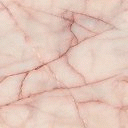
\includegraphics[height=3cm]{pink_marble.png}};
      \node[left,inner sep=0pt,outer sep=0pt] at (frame.east) {
\includegraphics[height=3cm]{crinklepaper.png}};
  },
  ]{name=title,column=1,span=3,below=top}{
  \resizebox{18cm}{!}{\bfseries\Huge My Important Project}\\[3mm]
  Hans.Mustermann@deepthought.university
}

%----
\posterbox[adjusted title=References]{name=references,column=2,span=1.5,above=bottom}{
}

%----
\posterbox[adjusted title=Process]{name=process,column=2,span=2,above=references}{
}

%----
\posterbox[adjusted title=Project Description]{name=project,
    sequence=1 between title and bottom then 2 between title and process}{
}

%----
\posterbox[adjusted title=Central Picture]
  {name=picture,column=3,between=title and process}{}

%----
\begin{posterboxenv}[adjusted title=Core Algorithm]
  {name=algorithm,column=4,between=top and references}
\end{posterboxenv}

%----
\posterbox[adjusted title=Contact]
    {name=contact,column*=4,span=1.5,between=process and bottom}{
}

\begin{posterboxenv}[blankest]{column=2,span=2,below=title,yshift=-5mm}
\begin{guide}[grow to left by=8mm,grow to right by=8mm,]
We make the \texttt{title} box different from the other boxes by removing
everything except the background. Also, two pictures are added left and
right which should be seen as logos or similar things.
\par\medskip

\begin{guidelisting}{}
%...
\posterbox[blankest,interior engine=path,height=3cm,
    halign=center,valign=center,fontupper=\bfseries\large,colupper=red!25!black,
    underlay={
      \node[right,inner sep=0pt,outer sep=0pt] at (frame.west) {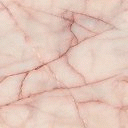
\includegraphics[height=3cm]{pink_marble.png}};
      \node[left,inner sep=0pt,outer sep=0pt] at (frame.east) {
\includegraphics[height=3cm]{crinklepaper.png}};
  },
  ]{name=title,column=1,span=3,below=top}{
  \resizebox{18cm}{!}{\bfseries\Huge My Important Project}\\[3mm]
  Hans.Mustermann@deepthought.university
}
%...
\end{guidelisting}
\end{guide}
\end{posterboxenv}
\end{tcbposter}




%%%%%%%%%%%%%%%%%%%%%%%%%%%%%%%%%%%%%%%%%%%%%%%%%%%%%%%%%%%%%%%%%%%%%%%%%%%%%%%
\begin{tcbposter}[
  coverage = {
      spread,
      interior style={top color=yellow,bottom color=yellow!50!red},
      watermark text={\LaTeX\ Poster},
      watermark color=yellow,
  },
  poster   = {showframe=false,columns=4,rows=5},
  boxes    = {
      enhanced standard jigsaw,sharp corners=downhill,arc=3mm,boxrule=1mm,
      colback=white,opacityback=0.75,colframe=blue,
      title style={left color=black,right color=cyan},
      fonttitle=\bfseries\Large\scshape
   }
]

%----
\posterbox[blankest,interior engine=path,height=3cm,
    halign=center,valign=center,fontupper=\bfseries\large,colupper=red!25!black,
    underlay={
      \node[right,inner sep=0pt,outer sep=0pt] at (frame.west) {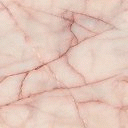
\includegraphics[height=3cm]{pink_marble.png}};
      \node[left,inner sep=0pt,outer sep=0pt] at (frame.east) {
\includegraphics[height=3cm]{crinklepaper.png}};
  },
  ]{name=title,column=1,span=3,below=top}{
  \resizebox{18cm}{!}{\bfseries\Huge My Important Project}\\[3mm]
  Hans.Mustermann@deepthought.university
}

%----
\posterbox[adjusted title=References]{name=references,column=2,span=1.5,above=bottom}{
  \begin{enumerate}[{[1]}]
  \item\label{litA} Important Authors, \textit{Important Title}
  \item\label{litB} More Important Authors, \textit{More Important Title}
  \item\label{litC} Less Important Authors, \textit{Less Important Title}
  \end{enumerate}
}

%----
\posterbox[adjusted title=Process]{name=process,column=2,span=2,above=references}{
}

%----
\posterbox[adjusted title=Project Description]{name=project,
    sequence=1 between title and bottom then 2 between title and process}{
}

%----
\posterbox[adjusted title=Central Picture]
  {name=picture,column=3,between=title and process}{}

%----
\begin{posterboxenv}[adjusted title=Core Algorithm]
  {name=algorithm,column=4,between=top and references}
\end{posterboxenv}

%----
\posterbox[adjusted title=Contact]
    {name=contact,column*=4,span=1.5,between=process and bottom}{
}

\begin{posterboxenv}[blankest]{column=2,span=2,above=references,yshift=5mm}
\begin{guide}
The \texttt{references} box is filled with a simple \texttt{enumerate} list.\par
You may insert a more fancier and \LaTeX ier bibliography for your real project \ldots
\par\medskip

\begin{guidelisting}{}
%...
\posterbox[adjusted title=References]{name=references,column=2,span=1.5,above=bottom}{
  \begin{enumerate}[{[1]}]
  \item\label{litA} Important Authors, \textit{Important Title}
  \item\label{litB} More Important Authors, \textit{More Important Title}
  \item\label{litC} Less Important Authors, \textit{Less Important Title}
  \end{enumerate}
}
%...
\end{guidelisting}
\medskip
Surely, you noted that all boxes adapt to the grown height of our
\texttt{references} box. Maybe, you want to get some pages back to see
how the box placements were done for this example.
\end{guide}
\end{posterboxenv}
\end{tcbposter}



%%%%%%%%%%%%%%%%%%%%%%%%%%%%%%%%%%%%%%%%%%%%%%%%%%%%%%%%%%%%%%%%%%%%%%%%%%%%%%%
\begin{tcbposter}[
  coverage = {
      spread,
      interior style={top color=yellow,bottom color=yellow!50!red},
      watermark text={\LaTeX\ Poster},
      watermark color=yellow,
  },
  poster   = {showframe=false,columns=4,rows=5},
  boxes    = {
      enhanced standard jigsaw,sharp corners=downhill,arc=3mm,boxrule=1mm,
      colback=white,opacityback=0.75,colframe=blue,
      title style={left color=black,right color=cyan},
      fonttitle=\bfseries\Large\scshape
   }
]

%----
\posterbox[blankest,interior engine=path,height=3cm,
    halign=center,valign=center,fontupper=\bfseries\large,colupper=red!25!black,
    underlay={
      \node[right,inner sep=0pt,outer sep=0pt] at (frame.west) {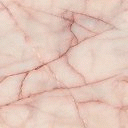
\includegraphics[height=3cm]{pink_marble.png}};
      \node[left,inner sep=0pt,outer sep=0pt] at (frame.east) {
\includegraphics[height=3cm]{crinklepaper.png}};
  },
  ]{name=title,column=1,span=3,below=top}{
  \resizebox{18cm}{!}{\bfseries\Huge My Important Project}\\[3mm]
  Hans.Mustermann@deepthought.university
}

%----
\posterbox[adjusted title=References]{name=references,column=2,span=1.5,above=bottom}{
  \begin{enumerate}[{[1]}]
  \item\label{litA} Important Authors, \textit{Important Title}
  \item\label{litB} More Important Authors, \textit{More Important Title}
  \item\label{litC} Less Important Authors, \textit{Less Important Title}
  \end{enumerate}
}

%----
\posterbox[adjusted title=Process,halign=center]{name=process,column=2,span=2,above=references}{
  
\begin{tikzpicture}[very thick,radius=2cm]
    \begin{scope}
      \path[draw=black,fill=white] (0,0) circle;
      \path[fill=red] (0,0) -- (2,0) arc [start angle=0, end angle=30];
    \end{scope}
    \begin{scope}[xshift=5cm]
      \path[draw=black,fill=white] (0,0) circle;
      \path[fill=red] (0,0) -- (2,0) arc [start angle=0, end angle=70];
    \end{scope}
    \begin{scope}[xshift=10cm]
      \path[draw=black,fill=white] (0,0) circle;
      \path[fill=red] (0,0) -- (2,0) arc [start angle=0, end angle=110];
    \end{scope}
    \begin{scope}[xshift=15cm]
      \path[draw=black,fill=white] (0,0) circle;
      \path[fill=red] (0,0) -- (2,0) arc [start angle=0, end angle=240];
    \end{scope}
  \end{tikzpicture}
}

%----
\posterbox[adjusted title=Project Description]{name=project,
    sequence=1 between title and bottom then 2 between title and process}{
}

%----
\posterbox[adjusted title=Central Picture]
  {name=picture,column=3,between=title and process}{}

%----
\begin{posterboxenv}[adjusted title=Core Algorithm]
  {name=algorithm,column=4,between=top and references}
\end{posterboxenv}

%----
\posterbox[adjusted title=Contact]
    {name=contact,column*=4,span=1.5,between=process and bottom}{
}

\begin{posterboxenv}[blankest]{column=2,span=2,above=process,yshift=5mm}
\begin{guide}
We go on with the \texttt{process} which gets some example \texttt{tikzpicture}.\par
Note that you always can insert additional \texttt{tcolorbox} options like
\texttt{halign=center} to a \texttt{posterbox}.
\par\medskip
\begin{guidelisting}{}
%...
\posterbox[adjusted title=Process,halign=center]{name=process,column=2,span=2,above=references}{
  
\begin{tikzpicture}[very thick,radius=2cm]
    \begin{scope}
      \path[draw=black,fill=white] (0,0) circle;
      \path[fill=red] (0,0) -- (2,0) arc [start angle=0, end angle=30];
    \end{scope}
    \begin{scope}[xshift=5cm]
      \path[draw=black,fill=white] (0,0) circle;
      \path[fill=red] (0,0) -- (2,0) arc [start angle=0, end angle=70];
    \end{scope}
    \begin{scope}[xshift=10cm]
      \path[draw=black,fill=white] (0,0) circle;
      \path[fill=red] (0,0) -- (2,0) arc [start angle=0, end angle=110];
    \end{scope}
    \begin{scope}[xshift=15cm]
      \path[draw=black,fill=white] (0,0) circle;
      \path[fill=red] (0,0) -- (2,0) arc [start angle=0, end angle=240];
    \end{scope}
  \end{tikzpicture}
}
%...
\end{guidelisting}
\end{guide}
\end{posterboxenv}
\end{tcbposter}




%%%%%%%%%%%%%%%%%%%%%%%%%%%%%%%%%%%%%%%%%%%%%%%%%%%%%%%%%%%%%%%%%%%%%%%%%%%%%%%
\begin{tcbposter}[
  coverage = {
      spread,
      interior style={top color=yellow,bottom color=yellow!50!red},
      watermark text={\LaTeX\ Poster},
      watermark color=yellow,
  },
  poster   = {showframe=false,columns=4,rows=5},
  boxes    = {
      enhanced standard jigsaw,sharp corners=downhill,arc=3mm,boxrule=1mm,
      colback=white,opacityback=0.75,colframe=blue,
      title style={left color=black,right color=cyan},
      fonttitle=\bfseries\Large\scshape
   }
]

%----
\posterbox[blankest,interior engine=path,height=3cm,
    halign=center,valign=center,fontupper=\bfseries\large,colupper=red!25!black,
    underlay={
      \node[right,inner sep=0pt,outer sep=0pt] at (frame.west) {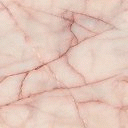
\includegraphics[height=3cm]{pink_marble.png}};
      \node[left,inner sep=0pt,outer sep=0pt] at (frame.east) {
\includegraphics[height=3cm]{crinklepaper.png}};
  },
  ]{name=title,column=1,span=3,below=top}{
  \resizebox{18cm}{!}{\bfseries\Huge My Important Project}\\[3mm]
  Hans.Mustermann@deepthought.university
}

%----
\posterbox[adjusted title=References]{name=references,column=2,span=1.5,above=bottom}{
  \begin{enumerate}[{[1]}]
  \item\label{litA} Important Authors, \textit{Important Title}
  \item\label{litB} More Important Authors, \textit{More Important Title}
  \item\label{litC} Less Important Authors, \textit{Less Important Title}
  \end{enumerate}
}

%----
\posterbox[adjusted title=Process,halign=center]{name=process,column=2,span=2,above=references}{
  
\begin{tikzpicture}[very thick,radius=2cm]
    \begin{scope}
      \path[draw=black,fill=white] (0,0) circle;
      \path[fill=red] (0,0) -- (2,0) arc [start angle=0, end angle=30];
    \end{scope}
    \begin{scope}[xshift=5cm]
      \path[draw=black,fill=white] (0,0) circle;
      \path[fill=red] (0,0) -- (2,0) arc [start angle=0, end angle=70];
    \end{scope}
    \begin{scope}[xshift=10cm]
      \path[draw=black,fill=white] (0,0) circle;
      \path[fill=red] (0,0) -- (2,0) arc [start angle=0, end angle=110];
    \end{scope}
    \begin{scope}[xshift=15cm]
      \path[draw=black,fill=white] (0,0) circle;
      \path[fill=red] (0,0) -- (2,0) arc [start angle=0, end angle=240];
    \end{scope}
  \end{tikzpicture}
}

%----
\posterbox[adjusted title=Project Description]{name=project,
    sequence=1 between title and bottom then 2 between title and process}{
  See [\ref{litA}]: \lipsum[1]
  \begin{center}
  \tikz \draw[thick,rounded corners=8pt]
    (0,0)--(0,2)--(1,3.25)--(2,2)--(2,0)--(0,2)--(2,2)--(0,0)--(2,0);
  \quad by [\ref{litB}]
  \end{center}
  \lipsum[2-3]\par
  See [\ref{litC}]:
  \lipsum[4]
  \begin{center}
  \tikz \shadedraw [left color=red,right color=blue]
  (0,0) rectangle (2,2);
  \end{center}
  That's all.
}

%----
\posterbox[adjusted title=Central Picture]
  {name=picture,column=3,between=title and process}{}

%----
\begin{posterboxenv}[adjusted title=Core Algorithm]
  {name=algorithm,column=4,between=top and references}
\end{posterboxenv}

%----
\posterbox[adjusted title=Contact]
    {name=contact,column*=4,span=1.5,between=process and bottom}{
}

\begin{posterboxenv}[blankest]{column=3,span=2,at=middle}
\begin{guide}
The \texttt{project} is a breakable box with two parts. Nevertheless,
you can fill the box like any other box. The information on how to
break was already given by the placement options.

\par\medskip
\begin{guidelisting}{}
%...
\posterbox[adjusted title=Project Description]{name=project,
    sequence=1 between title and bottom then 2 between title and process}{
  See [\ref{litA}]: \lipsum[1]
  \begin{center}
  \tikz \draw[thick,rounded corners=8pt]
    (0,0)--(0,2)--(1,3.25)--(2,2)--(2,0)--(0,2)--(2,2)--(0,0)--(2,0);
  \quad by [\ref{litB}]
  \end{center}
  \lipsum[2-3]\par
  See [\ref{litC}]:
  \lipsum[4]
  \begin{center}
  \tikz \shadedraw [left color=red,right color=blue]
  (0,0) rectangle (2,2);
  \end{center}
  That's all.
}
%...
\end{guidelisting}
\medskip
The two boxes have a \emph{closed} appearance, because we used
\texttt{enhanced standard jigsaw} as global style for all boxes.
For an \emph{open} appearance, just use \texttt{enhanced jigsaw} instead:\par\medskip
\begin{guidelisting}{}
%...
\begin{tcbposter}[
%...
  boxes    = {
      enhanced jigsaw,% <-----------
      sharp corners=downhill,arc=3mm,boxrule=1mm,
%...
   }
]
%...
\end{guidelisting}
\end{guide}
\end{posterboxenv}
\end{tcbposter}



%%%%%%%%%%%%%%%%%%%%%%%%%%%%%%%%%%%%%%%%%%%%%%%%%%%%%%%%%%%%%%%%%%%%%%%%%%%%%%%
\begin{tcbposter}[
  coverage = {
      spread,
      interior style={top color=yellow,bottom color=yellow!50!red},
      watermark text={\LaTeX\ Poster},
      watermark color=yellow,
  },
  poster   = {showframe=false,columns=4,rows=5},
  boxes    = {
      enhanced standard jigsaw,sharp corners=downhill,arc=3mm,boxrule=1mm,
      colback=white,opacityback=0.75,colframe=blue,
      title style={left color=black,right color=cyan},
      fonttitle=\bfseries\Large\scshape
   }
]

%----
\posterbox[blankest,interior engine=path,height=3cm,
    halign=center,valign=center,fontupper=\bfseries\large,colupper=red!25!black,
    underlay={
      \node[right,inner sep=0pt,outer sep=0pt] at (frame.west) {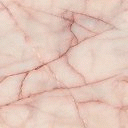
\includegraphics[height=3cm]{pink_marble.png}};
      \node[left,inner sep=0pt,outer sep=0pt] at (frame.east) {
\includegraphics[height=3cm]{crinklepaper.png}};
  },
  ]{name=title,column=1,span=3,below=top}{
  \resizebox{18cm}{!}{\bfseries\Huge My Important Project}\\[3mm]
  Hans.Mustermann@deepthought.university
}

%----
\posterbox[adjusted title=References]{name=references,column=2,span=1.5,above=bottom}{
  \begin{enumerate}[{[1]}]
  \item\label{litA} Important Authors, \textit{Important Title}
  \item\label{litB} More Important Authors, \textit{More Important Title}
  \item\label{litC} Less Important Authors, \textit{Less Important Title}
  \end{enumerate}
}

%----
\posterbox[adjusted title=Process,halign=center]{name=process,column=2,span=2,above=references}{
  
\begin{tikzpicture}[very thick,radius=2cm]
    \begin{scope}
      \path[draw=black,fill=white] (0,0) circle;
      \path[fill=red] (0,0) -- (2,0) arc [start angle=0, end angle=30];
    \end{scope}
    \begin{scope}[xshift=5cm]
      \path[draw=black,fill=white] (0,0) circle;
      \path[fill=red] (0,0) -- (2,0) arc [start angle=0, end angle=70];
    \end{scope}
    \begin{scope}[xshift=10cm]
      \path[draw=black,fill=white] (0,0) circle;
      \path[fill=red] (0,0) -- (2,0) arc [start angle=0, end angle=110];
    \end{scope}
    \begin{scope}[xshift=15cm]
      \path[draw=black,fill=white] (0,0) circle;
      \path[fill=red] (0,0) -- (2,0) arc [start angle=0, end angle=240];
    \end{scope}
  \end{tikzpicture}
}

%----
\posterbox[adjusted title=Project Description]{name=project,
    sequence=1 between title and bottom then 2 between title and process}{
  See [\ref{litA}]: \lipsum[1]
  \begin{center}
  \tikz \draw[thick,rounded corners=8pt]
    (0,0)--(0,2)--(1,3.25)--(2,2)--(2,0)--(0,2)--(2,2)--(0,0)--(2,0);
  \quad by [\ref{litB}]
  \end{center}
  \lipsum[2-3]\par
  See [\ref{litC}]:
  \lipsum[4]
  \begin{center}
  \tikz \shadedraw [left color=red,right color=blue]
  (0,0) rectangle (2,2);
  \end{center}
  That's all.
}

%----
\posterbox[adjusted title=Central Picture,
  interior style={fill overzoom image=blueshade.png}]
  {name=picture,column=3,between=title and process}{}

%----
\begin{posterboxenv}[adjusted title=Core Algorithm]
  {name=algorithm,column=4,between=top and references}
\end{posterboxenv}

%----
\posterbox[adjusted title=Contact]
    {name=contact,column*=4,span=1.5,between=process and bottom}{
}

\begin{posterboxenv}[blankest]{column=2,span=2,below=picture,yshift=-5mm}
\begin{guide}
In our example, the whole space of the \texttt{picture} box should be
filled with a given picture. This is a piece of cake using a special
\texttt{interior style}:
\par\medskip
\begin{guidelisting}{}
%...
\posterbox[adjusted title=Central Picture,
  interior style={fill overzoom image=blueshade.png}]
  {name=picture,column=3,between=title and process}{}
%...
\end{guidelisting}
\end{guide}
\end{posterboxenv}
\end{tcbposter}



\begin{tcbverbatimwrite}{\jobname.mylist}
%...
\begin{posterboxenv}[adjusted title=Core Algorithm,leftupper=0pt,rightupper=0pt]
  {name=algorithm,column=4,between=top and references}
\begin{tcblisting}{blankest,listing only}
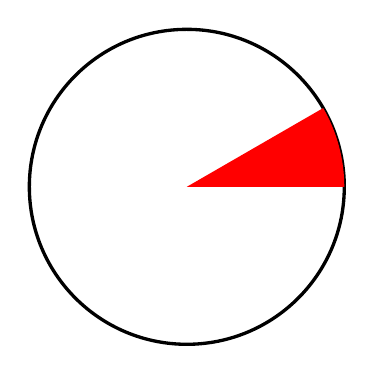
\begin{tikzpicture}[very thick,radius=2cm]
  \begin{scope}
    \path[draw=black,fill=white] (0,0) circle;
    \path[fill=red] (0,0) -- (2,0)
      arc [start angle=0, end angle=30];
  \end{scope}
%...
\end{tikzpicture}
\end{tcblisting}
\end{posterboxenv}
%...
\end{tcbverbatimwrite}

%%%%%%%%%%%%%%%%%%%%%%%%%%%%%%%%%%%%%%%%%%%%%%%%%%%%%%%%%%%%%%%%%%%%%%%%%%%%%%%
\begin{tcbposter}[
  coverage = {
      spread,
      interior style={top color=yellow,bottom color=yellow!50!red},
      watermark text={\LaTeX\ Poster},
      watermark color=yellow,
  },
  poster   = {showframe=false,columns=4,rows=5},
  boxes    = {
      enhanced standard jigsaw,sharp corners=downhill,arc=3mm,boxrule=1mm,
      colback=white,opacityback=0.75,colframe=blue,
      title style={left color=black,right color=cyan},
      fonttitle=\bfseries\Large\scshape
   }
]

%----
\posterbox[blankest,interior engine=path,height=3cm,
    halign=center,valign=center,fontupper=\bfseries\large,colupper=red!25!black,
    underlay={
      \node[right,inner sep=0pt,outer sep=0pt] at (frame.west) {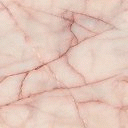
\includegraphics[height=3cm]{pink_marble.png}};
      \node[left,inner sep=0pt,outer sep=0pt] at (frame.east) {
\includegraphics[height=3cm]{crinklepaper.png}};
  },
  ]{name=title,column=1,span=3,below=top}{
  \resizebox{18cm}{!}{\bfseries\Huge My Important Project}\\[3mm]
  Hans.Mustermann@deepthought.university
}

%----
\posterbox[adjusted title=References]{name=references,column=2,span=1.5,above=bottom}{
  \begin{enumerate}[{[1]}]
  \item\label{litA} Important Authors, \textit{Important Title}
  \item\label{litB} More Important Authors, \textit{More Important Title}
  \item\label{litC} Less Important Authors, \textit{Less Important Title}
  \end{enumerate}
}

%----
\posterbox[adjusted title=Process,halign=center]{name=process,column=2,span=2,above=references}{
  
\begin{tikzpicture}[very thick,radius=2cm]
    \begin{scope}
      \path[draw=black,fill=white] (0,0) circle;
      \path[fill=red] (0,0) -- (2,0) arc [start angle=0, end angle=30];
    \end{scope}
    \begin{scope}[xshift=5cm]
      \path[draw=black,fill=white] (0,0) circle;
      \path[fill=red] (0,0) -- (2,0) arc [start angle=0, end angle=70];
    \end{scope}
    \begin{scope}[xshift=10cm]
      \path[draw=black,fill=white] (0,0) circle;
      \path[fill=red] (0,0) -- (2,0) arc [start angle=0, end angle=110];
    \end{scope}
    \begin{scope}[xshift=15cm]
      \path[draw=black,fill=white] (0,0) circle;
      \path[fill=red] (0,0) -- (2,0) arc [start angle=0, end angle=240];
    \end{scope}
  \end{tikzpicture}
}

%----
\posterbox[adjusted title=Project Description]{name=project,
    sequence=1 between title and bottom then 2 between title and process}{
  See [\ref{litA}]: \lipsum[1]
  \begin{center}
  \tikz \draw[thick,rounded corners=8pt]
    (0,0)--(0,2)--(1,3.25)--(2,2)--(2,0)--(0,2)--(2,2)--(0,0)--(2,0);
  \quad by [\ref{litB}]
  \end{center}
  \lipsum[2-3]\par
  See [\ref{litC}]:
  \lipsum[4]
  \begin{center}
  \tikz \shadedraw [left color=red,right color=blue]
  (0,0) rectangle (2,2);
  \end{center}
  That's all.
}

%----
\posterbox[adjusted title=Central Picture,
  interior style={fill overzoom image=blueshade.png}]
  {name=picture,column=3,between=title and process}{}

%----
\begin{posterboxenv}[adjusted title=Core Algorithm,leftupper=0pt,rightupper=0pt]
  {name=algorithm,column=4,between=top and references}
\begin{tcblisting}{blankest,listing only}

\begin{tikzpicture}[very thick,radius=2cm]
  \begin{scope}
    \path[draw=black,fill=white] (0,0) circle;
    \path[fill=red] (0,0) -- (2,0)
      arc [start angle=0, end angle=30];
  \end{scope}
  \begin{scope}[xshift=5cm]
    \path[draw=black,fill=white] (0,0) circle;
    \path[fill=red] (0,0) -- (2,0)
      arc [start angle=0, end angle=70];
  \end{scope}
  \begin{scope}[xshift=10cm]
    \path[draw=black,fill=white] (0,0) circle;
    \path[fill=red] (0,0) -- (2,0)
      arc [start angle=0, end angle=110];
  \end{scope}
  \begin{scope}[xshift=15cm]
    \path[draw=black,fill=white] (0,0) circle;
    \path[fill=red] (0,0) -- (2,0)
      arc [start angle=0, end angle=240];
  \end{scope}
\end{tikzpicture}

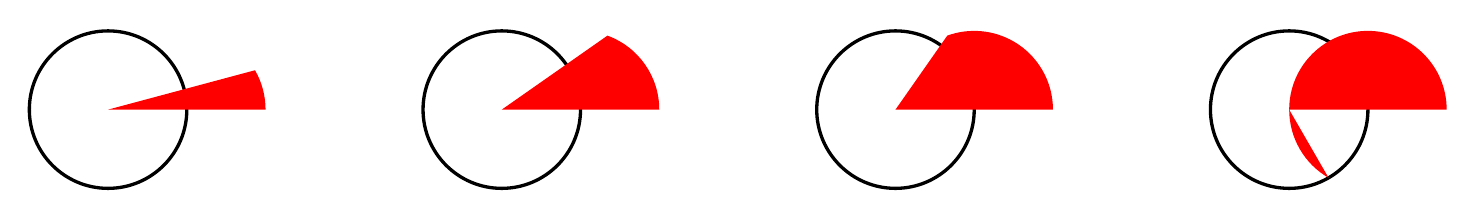
\begin{tikzpicture}[very thick,radius=1cm]
  \begin{scope}
    \path[draw=black,fill=white] (0,0) circle;
    \path[fill=red] (0,0) -- (2,0)
      arc [start angle=0, end angle=30];
  \end{scope}
  \begin{scope}[xshift=5cm]
    \path[draw=black,fill=white] (0,0) circle;
    \path[fill=red] (0,0) -- (2,0)
      arc [start angle=0, end angle=70];
  \end{scope}
  \begin{scope}[xshift=10cm]
    \path[draw=black,fill=white] (0,0) circle;
    \path[fill=red] (0,0) -- (2,0)
      arc [start angle=0, end angle=110];
  \end{scope}
  \begin{scope}[xshift=15cm]
    \path[draw=black,fill=white] (0,0) circle;
    \path[fill=red] (0,0) -- (2,0)
      arc [start angle=0, end angle=240];
  \end{scope}
\end{tikzpicture}
\end{tcblisting}
\end{posterboxenv}

%----
\posterbox[adjusted title=Contact]
    {name=contact,column*=4,span=1.5,between=process and bottom}{
}

\begin{posterboxenv}[blankest]{column=2,span=2,below=picture,at=middle}
\begin{guide}
For the Algorithm, we need a \texttt{verbatim} environment. Here,
\texttt{tcblisting} is used.\par
Therefore, we cannot use a \texttt{posterbox} as usual, but we can
a \texttt{posterboxenv} environment instead.\par
Note that you would get some weird errors, if \texttt{posterbox} would have been applied.
\par\medskip
\tcbinputlisting{mylisting,listing file=\jobname.mylist}
\end{guide}
\end{posterboxenv}
\end{tcbposter}




%%%%%%%%%%%%%%%%%%%%%%%%%%%%%%%%%%%%%%%%%%%%%%%%%%%%%%%%%%%%%%%%%%%%%%%%%%%%%%%

\begin{tcbposter}[
  coverage = {
      spread,
      interior style={top color=yellow,bottom color=yellow!50!red},
      watermark text={\LaTeX\ Poster},
      watermark color=yellow,
  },
  poster   = {showframe=false,columns=4,rows=5},
  boxes    = {
      enhanced standard jigsaw,sharp corners=downhill,arc=3mm,boxrule=1mm,
      colback=white,opacityback=0.75,colframe=blue,
      title style={left color=black,right color=cyan},
      fonttitle=\bfseries\Large\scshape
   }
]

%----
\posterbox[blankest,interior engine=path,height=3cm,
    halign=center,valign=center,fontupper=\bfseries\large,colupper=red!25!black,
    underlay={
      \node[right,inner sep=0pt,outer sep=0pt] at (frame.west) {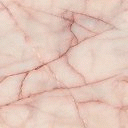
\includegraphics[height=3cm]{pink_marble.png}};
      \node[left,inner sep=0pt,outer sep=0pt] at (frame.east) {
\includegraphics[height=3cm]{crinklepaper.png}};
  },
  ]{name=title,column=1,span=3,below=top}{
  \resizebox{18cm}{!}{\bfseries\Huge My Important Project}\\[3mm]
  Hans.Mustermann@deepthought.university
}

%----
\posterbox[adjusted title=References]{name=references,column=2,span=1.5,above=bottom}{
  \begin{enumerate}[{[1]}]
  \item\label{litA} Important Authors, \textit{Important Title}
  \item\label{litB} More Important Authors, \textit{More Important Title}
  \item\label{litC} Less Important Authors, \textit{Less Important Title}
  \end{enumerate}
}

%----
\posterbox[adjusted title=Process,halign=center]{name=process,column=2,span=2,above=references}{
  
\begin{tikzpicture}[very thick,radius=2cm]
    \begin{scope}
      \path[draw=black,fill=white] (0,0) circle;
      \path[fill=red] (0,0) -- (2,0) arc [start angle=0, end angle=30];
    \end{scope}
    \begin{scope}[xshift=5cm]
      \path[draw=black,fill=white] (0,0) circle;
      \path[fill=red] (0,0) -- (2,0) arc [start angle=0, end angle=70];
    \end{scope}
    \begin{scope}[xshift=10cm]
      \path[draw=black,fill=white] (0,0) circle;
      \path[fill=red] (0,0) -- (2,0) arc [start angle=0, end angle=110];
    \end{scope}
    \begin{scope}[xshift=15cm]
      \path[draw=black,fill=white] (0,0) circle;
      \path[fill=red] (0,0) -- (2,0) arc [start angle=0, end angle=240];
    \end{scope}
  \end{tikzpicture}
}

%----
\posterbox[adjusted title=Project Description]{name=project,
    sequence=1 between title and bottom then 2 between title and process}{
  See [\ref{litA}]: \lipsum[1]
  \begin{center}
  \tikz \draw[thick,rounded corners=8pt]
    (0,0)--(0,2)--(1,3.25)--(2,2)--(2,0)--(0,2)--(2,2)--(0,0)--(2,0);
  \quad by [\ref{litB}]
  \end{center}
  \lipsum[2-3]\par
  See [\ref{litC}]:
  \lipsum[4]
  \begin{center}
  \tikz \shadedraw [left color=red,right color=blue]
  (0,0) rectangle (2,2);
  \end{center}
  That's all.
}

%----
\posterbox[adjusted title=Central Picture,
  interior style={fill overzoom image=blueshade.png}]
  {name=picture,column=3,between=title and process}{}

%----
\begin{posterboxenv}[adjusted title=Core Algorithm,leftupper=0pt,rightupper=0pt]
  {name=algorithm,column=4,between=top and references}
\begin{tcblisting}{blankest,listing only}

\begin{tikzpicture}[very thick,radius=2cm]
  \begin{scope}
    \path[draw=black,fill=white] (0,0) circle;
    \path[fill=red] (0,0) -- (2,0)
      arc [start angle=0, end angle=30];
  \end{scope}
  \begin{scope}[xshift=5cm]
    \path[draw=black,fill=white] (0,0) circle;
    \path[fill=red] (0,0) -- (2,0)
      arc [start angle=0, end angle=70];
  \end{scope}
  \begin{scope}[xshift=10cm]
    \path[draw=black,fill=white] (0,0) circle;
    \path[fill=red] (0,0) -- (2,0)
      arc [start angle=0, end angle=110];
  \end{scope}
  \begin{scope}[xshift=15cm]
    \path[draw=black,fill=white] (0,0) circle;
    \path[fill=red] (0,0) -- (2,0)
      arc [start angle=0, end angle=240];
  \end{scope}
\end{tikzpicture}

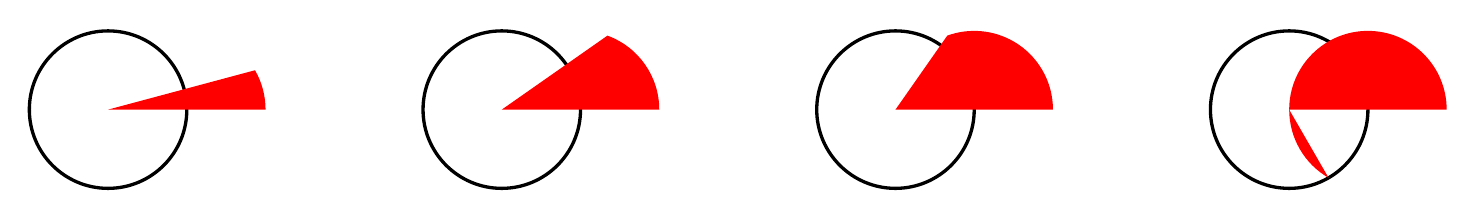
\begin{tikzpicture}[very thick,radius=1cm]
  \begin{scope}
    \path[draw=black,fill=white] (0,0) circle;
    \path[fill=red] (0,0) -- (2,0)
      arc [start angle=0, end angle=30];
  \end{scope}
  \begin{scope}[xshift=5cm]
    \path[draw=black,fill=white] (0,0) circle;
    \path[fill=red] (0,0) -- (2,0)
      arc [start angle=0, end angle=70];
  \end{scope}
  \begin{scope}[xshift=10cm]
    \path[draw=black,fill=white] (0,0) circle;
    \path[fill=red] (0,0) -- (2,0)
      arc [start angle=0, end angle=110];
  \end{scope}
  \begin{scope}[xshift=15cm]
    \path[draw=black,fill=white] (0,0) circle;
    \path[fill=red] (0,0) -- (2,0)
      arc [start angle=0, end angle=240];
  \end{scope}
\end{tikzpicture}
\end{tcblisting}
\end{posterboxenv}

%----
\posterbox[adjusted title=Contact,fit,fit basedim=12pt]
    {name=contact,column*=4,span=1.5,between=process and bottom}{
  \lipsum[2]
}

\begin{posterboxenv}[blankest]{column=2,span=2,above=contact,yshift=5mm}
\begin{guide}
Finally, the \texttt{contact} box is filled. But, in our example case,
there is not much space for a lot of contact text.\par
Therefore, we add \texttt{fit} to fit in the text automatically.
\par\medskip
\begin{guidelisting}{}
%...
\posterbox[adjusted title=Contact,fit,fit basedim=12pt]
    {name=contact,column*=4,span=1.5,between=process and bottom}{
  \lipsum[2]
}
%...
\end{guidelisting}
\par\medskip
Our poster is finished now. Just go to the next page to see the final result.
\end{guide}
\end{posterboxenv}

\end{tcbposter}

%%%%%%%%%%%%%%%%%%%%%%%%%%%%%%%%%%%%%%%%%%%%%%%%%%%%%%%%%%%%%%%%%%%%%%%%%%%%%%%
\begin{tcbposter}[
  coverage = {
      spread,
      interior style={top color=yellow,bottom color=yellow!50!red},
      watermark text={\LaTeX\ Poster},
      watermark color=yellow,
  },
  poster   = {showframe=false,columns=4,rows=5},
  boxes    = {
      enhanced standard jigsaw,sharp corners=downhill,arc=3mm,boxrule=1mm,
      colback=white,opacityback=0.75,colframe=blue,
      title style={left color=black,right color=cyan},
      fonttitle=\bfseries\Large\scshape
   }
]

%----
\posterbox[blankest,interior engine=path,height=3cm,
    halign=center,valign=center,fontupper=\bfseries\large,colupper=red!25!black,
    underlay={
      \node[right,inner sep=0pt,outer sep=0pt] at (frame.west) {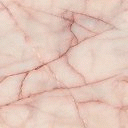
\includegraphics[height=3cm]{pink_marble.png}};
      \node[left,inner sep=0pt,outer sep=0pt] at (frame.east) {
\includegraphics[height=3cm]{crinklepaper.png}};
  },
  ]{name=title,column=1,span=3,below=top}{
  \resizebox{18cm}{!}{\bfseries\Huge My Important Project}\\[3mm]
  Hans.Mustermann@deepthought.university
}

%----
\posterbox[adjusted title=References]{name=references,column=2,span=1.5,above=bottom}{
  \begin{enumerate}[{[1]}]
  \item\label{litA} Important Authors, \textit{Important Title}
  \item\label{litB} More Important Authors, \textit{More Important Title}
  \item\label{litC} Less Important Authors, \textit{Less Important Title}
  \end{enumerate}
}

%----
\posterbox[adjusted title=Process,halign=center]{name=process,column=2,span=2,above=references}{
  
\begin{tikzpicture}[very thick,radius=2cm]
    \begin{scope}
      \path[draw=black,fill=white] (0,0) circle;
      \path[fill=red] (0,0) -- (2,0) arc [start angle=0, end angle=30];
    \end{scope}
    \begin{scope}[xshift=5cm]
      \path[draw=black,fill=white] (0,0) circle;
      \path[fill=red] (0,0) -- (2,0) arc [start angle=0, end angle=70];
    \end{scope}
    \begin{scope}[xshift=10cm]
      \path[draw=black,fill=white] (0,0) circle;
      \path[fill=red] (0,0) -- (2,0) arc [start angle=0, end angle=110];
    \end{scope}
    \begin{scope}[xshift=15cm]
      \path[draw=black,fill=white] (0,0) circle;
      \path[fill=red] (0,0) -- (2,0) arc [start angle=0, end angle=240];
    \end{scope}
  \end{tikzpicture}
}

%----
\posterbox[adjusted title=Project Description]{name=project,
    sequence=1 between title and bottom then 2 between title and process}{
  See [\ref{litA}]: \lipsum[1]
  \begin{center}
  \tikz \draw[thick,rounded corners=8pt]
    (0,0)--(0,2)--(1,3.25)--(2,2)--(2,0)--(0,2)--(2,2)--(0,0)--(2,0);
  \quad by [\ref{litB}]
  \end{center}
  \lipsum[2-3]\par
  See [\ref{litC}]:
  \lipsum[4]
  \begin{center}
  \tikz \shadedraw [left color=red,right color=blue]
  (0,0) rectangle (2,2);
  \end{center}
  That's all.
}

%----
\posterbox[adjusted title=Central Picture,
  interior style={fill overzoom image=blueshade.png}]
  {name=picture,column=3,between=title and process}{}

%----
\begin{posterboxenv}[adjusted title=Core Algorithm,leftupper=0pt,rightupper=0pt]
  {name=algorithm,column=4,between=top and references}
\begin{tcblisting}{blankest,listing only}

\begin{tikzpicture}[very thick,radius=2cm]
  \begin{scope}
    \path[draw=black,fill=white] (0,0) circle;
    \path[fill=red] (0,0) -- (2,0)
      arc [start angle=0, end angle=30];
  \end{scope}
  \begin{scope}[xshift=5cm]
    \path[draw=black,fill=white] (0,0) circle;
    \path[fill=red] (0,0) -- (2,0)
      arc [start angle=0, end angle=70];
  \end{scope}
  \begin{scope}[xshift=10cm]
    \path[draw=black,fill=white] (0,0) circle;
    \path[fill=red] (0,0) -- (2,0)
      arc [start angle=0, end angle=110];
  \end{scope}
  \begin{scope}[xshift=15cm]
    \path[draw=black,fill=white] (0,0) circle;
    \path[fill=red] (0,0) -- (2,0)
      arc [start angle=0, end angle=240];
  \end{scope}
\end{tikzpicture}

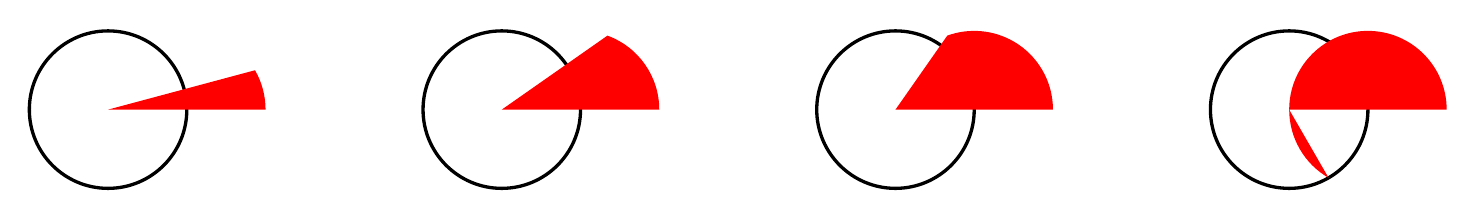
\begin{tikzpicture}[very thick,radius=1cm]
  \begin{scope}
    \path[draw=black,fill=white] (0,0) circle;
    \path[fill=red] (0,0) -- (2,0)
      arc [start angle=0, end angle=30];
  \end{scope}
  \begin{scope}[xshift=5cm]
    \path[draw=black,fill=white] (0,0) circle;
    \path[fill=red] (0,0) -- (2,0)
      arc [start angle=0, end angle=70];
  \end{scope}
  \begin{scope}[xshift=10cm]
    \path[draw=black,fill=white] (0,0) circle;
    \path[fill=red] (0,0) -- (2,0)
      arc [start angle=0, end angle=110];
  \end{scope}
  \begin{scope}[xshift=15cm]
    \path[draw=black,fill=white] (0,0) circle;
    \path[fill=red] (0,0) -- (2,0)
      arc [start angle=0, end angle=240];
  \end{scope}
\end{tikzpicture}
\end{tcblisting}
\end{posterboxenv}

%----
\posterbox[adjusted title=Contact,fit,fit basedim=12pt]
    {name=contact,column*=4,span=1.5,between=process and bottom}{
  \lipsum[2]
}

\end{tcbposter}


%%%%%%%%%%%%%%%%%%%%%%%%%%%%%%%%%%%%%%%%%%%%%%%%%%%%%%%%%%%%%%%%%%%%%%%%%%%%%%%
\begin{tcbposter}[
  coverage = {
      spread,
      interior style={top color=yellow,bottom color=yellow!50!red},
      watermark text={\LaTeX\ Poster},
      watermark color=yellow,
  },
  poster   = {showframe=false,columns=3,rows=5},
]

%----
\posterbox[blankest]{name=title,column=1,span=1,below=top}{
  \begin{guide}[grow to left by=0mm,grow to right by=-16mm]
  Source code for the example poster
  \end{guide}
}
\posterbox[blankest,posterset/fontsize=11pt]{name=source,
    sequence=1 between title and bottom then
             2 between top and bottom then
             3 between top and bottom
        }{%
    \tcbinputlisting{standard jigsaw,size=minimal,toprule=0.5mm,bottomrule=0.5mm,boxsep=2mm,
      colback=white,opacityback=0.75,listing only,
      enforce breakable,tcb@poster@boxheight,before skip=-\interlineskip,height fixed for=all,
      minted options={tabsize=2,fontsize=\small,breaklines,breakafter={,]-}},
      listing file=tcolorbox-example-poster.tex}%
  }
\end{tcbposter}


\end{document}

